\documentclass{article}
\usepackage[utf8]{inputenc}
\usepackage{graphicx}
\usepackage{listings}
\lstset{showstringspaces=false}
%Path relative to the .tex file containing the \includegraphics command
\graphicspath{ {images/} }

\title{Our first open source contribution.}
\author{Efthymia Kostaki \\
	 \texttt{ t8170055@aueb.gr}
	 \and
	 Stergios Sozos \\
 	 \texttt{t8170129@aueb.gr}
}
\date{May 2020}

\begin{document}
\maketitle

\begin{abstract}
The procedure of contributing to an open-source project was unique and unlike anything we have done before. All the phases for this assignment, from researching for the open-source project to selecting one and starting working on it, urged us to 
work more professionally and to create production-ready code.
\end{abstract}

% Image
\begin{figure}[tph!]
\centerline{
\includegraphics[totalheight=3cm, width= 10cm]{anitab-logo.png}}
    \caption{AnitaB [1]}
    \label{fig:verticalcell}
\end{figure}
%-----

% Image
\begin{figure}[tph!]
\centerline{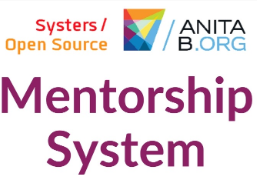
\includegraphics[totalheight=4cm, width= 4cm]{mentorship-system-logo.png}}
    \caption{MentorshipSystem[2]}
    \label{fig:verticalcell}
\end{figure}
%-----
\newpage

\tableofcontents

\newpage

\section*{Introduction}
The methodology we used for this assignment can be split into two main parts. Firstly, in the selection of the open-source project we worked in a structured way, so we did research individually in projetcs of our interests and focused in specific programming languages. We categorized our findings and decided on the project. The second part is how we worked in the open-source project itself. We worked on already made issues and issues we identified.  Each one of us was assigned to a specific issue, and he/ she undertook namely all the work on this issue, regarding branching, writing, communicating, opening a Pull Request and solving changes required using Github. For solving each of the issues mentioned we worked together, via Teamviewer, we agreed and implemented  all the changes we would propose. All the chages we are suggesting and discussions are available on Github in the specific issues we are mentioning.

\section{Project Selection Process}

\hspace{0.5cm}We utilized all the resources for finding an Open Source Project and we found more useful for us the site CodeTriage where we could explore different projects according to their programming language. Also, it was really important for us that the project we would choose would have an impact in the society.
We organized the projects according to the frequency of updates, the variety of contribution from different nationalities, gender etc. and how often where pull requests accepted, issues generated, if there were issues for first-time contributors and the number of pull requests needing review versus the ones closed or accepted. These metrics helped us understand if a project was `alive` and if it was interesting for us to work on it. We focused mainly in JAVA and Python. 

We chose three of these OSS projects to install and build and also discussed with Mr Gkortzis our choices and their implementation. Due to operation system requirements (Windows) we disregarded one of them, Pretix, and focused on the other two. We successfully built Mentorship Backend and that’s the project we worked on.

To sum up, the reasons why we chose Mentorship Backend are these:
\begin{itemize}
  \item Python language 
  \item Use of Google Python Style Guide,
  \item Guidance with resources for contributing and  Commit Message Style Guide,
  \item Communication on a daily basis on zulip chat using different communication channels for each problem,
  \item Focus on issues for First Timers,
  \item Meaningful impact in mentoring women in tech,
  \item Interested in trying to contribute to the project also on the Android development part.
\end{itemize}

\subsection{Troubleshooting}
Of course, we were not able to build the projects immidiately since we had some setup problems. We asked the community on Zulip to guide us through this process and if they knew how to solve our problems. Here is the questions we asked summarized:


% Image
\begin{figure}[tph!]
\centerline{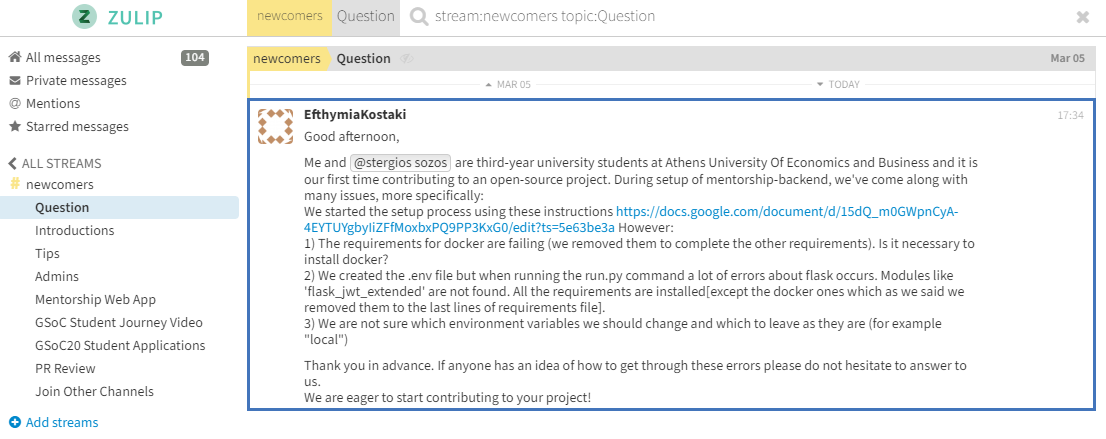
\includegraphics[totalheight=8cm, width=18cm]{Setup-problems.png}}
    \caption{Setup Problems}
    \label{fig:verticalcell}
\end{figure}
%-----

After a vary insightful discussion with the community we were able to build the project and also share our insights in how we solved these problems if a new contributor wants to set up this project!
% Image
\begin{figure}[tph!]
\centerline{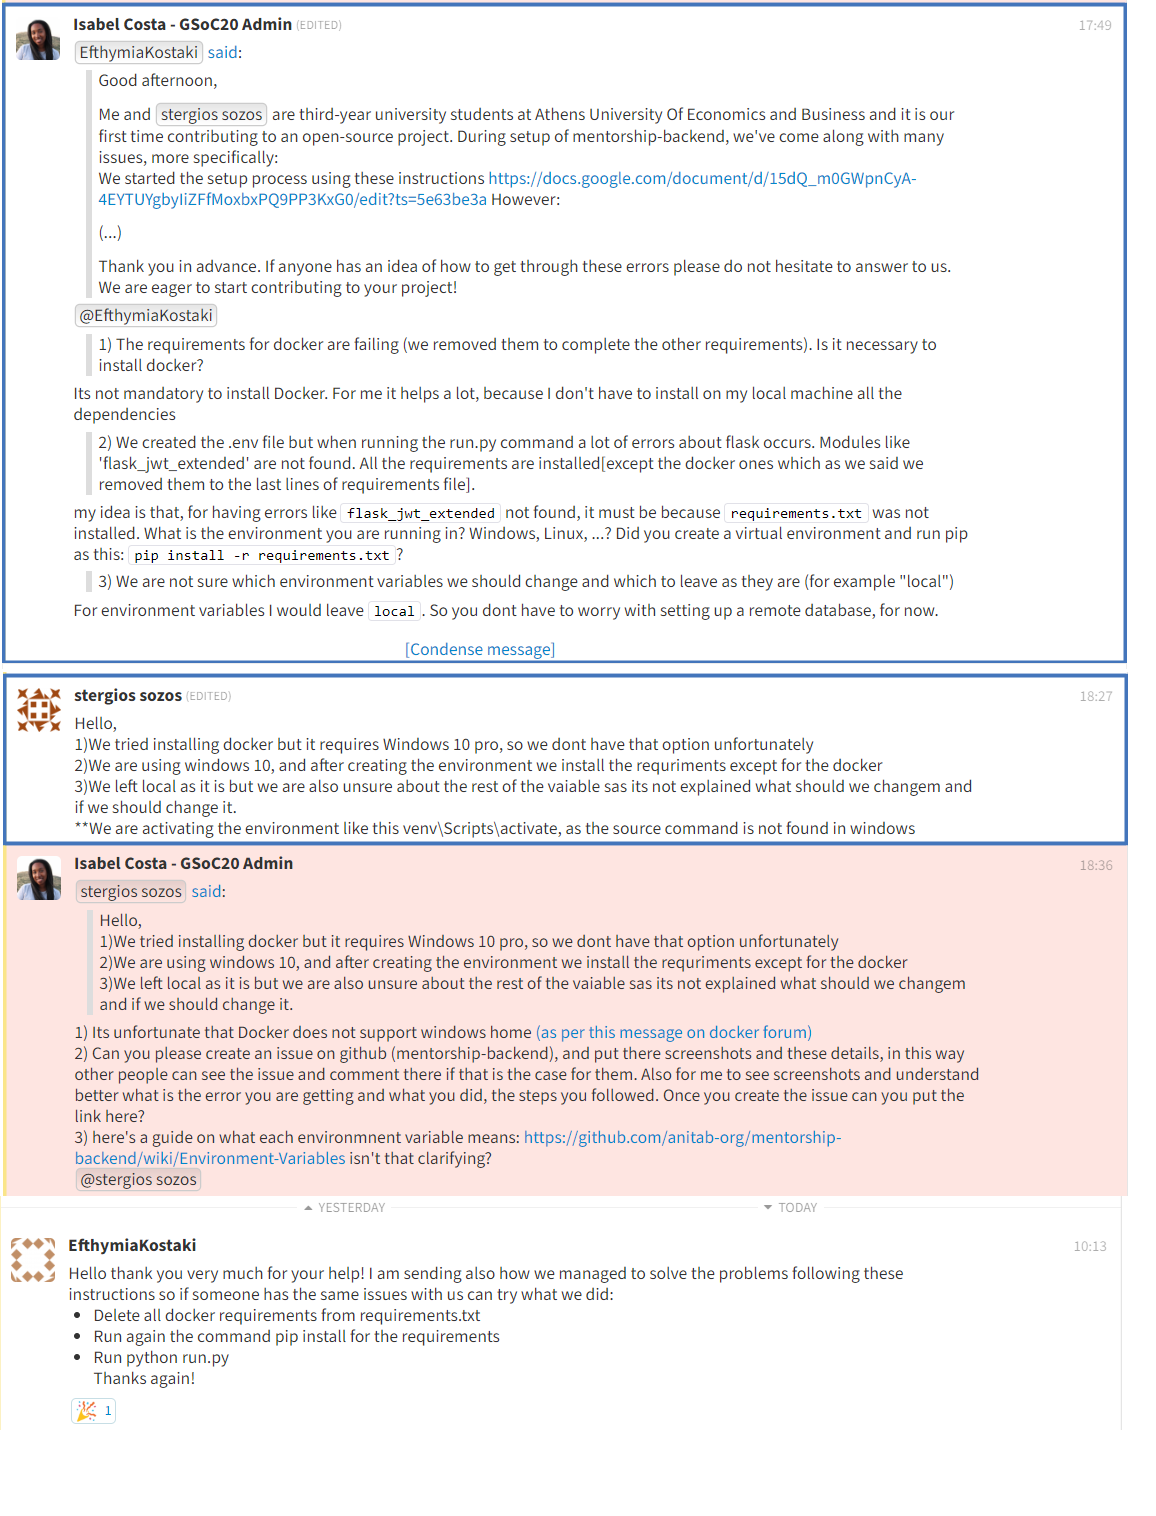
\includegraphics[totalheight=16cm, width=16cm]{Setup-discussion.png}}
    \caption{Setup Discussion}
    \label{fig:verticalcell}
\end{figure}
%-----

\vfill
\clearpage

\section{Mentorship Backend}

\hspace{0.5cm}Mentorship System is an application that matches women in tech to mentor each other, on career development, through 1:1 relations during a certain period of time. The project is deplyed in Heroku in this link: https://mentorship-backend-temp.herokuapp.com/. The backend is based on a REST API. There is also the Android client of the app for creating the interface for the users. [3]

The repository has the following permanent branches:
\begin{itemize}
 \item \textbf{master}: This contains the code which has been released.
 \item \textbf{develop}: This contains the latest code. All the contributing PRs must be sent to this branch. When we want to release the next version of the app, this branch is merged into the master branch. 
\end{itemize}

\section{Initial Communication with the community}
% Image
\begin{figure}[tph!]
\centerline{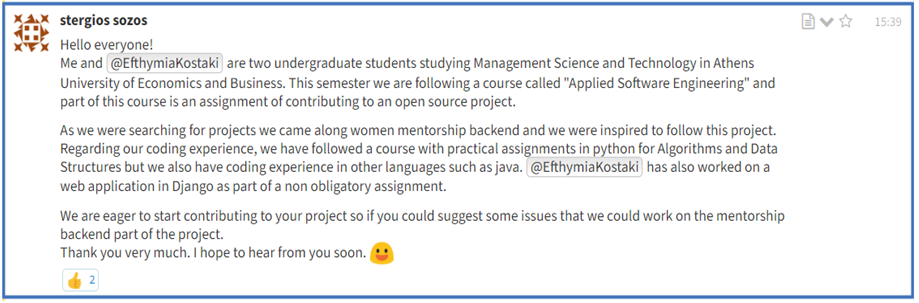
\includegraphics[totalheight=5cm]{FirstCommunication.png}}
    \caption{First Communication}
    \label{fig:verticalcell}
\end{figure}
%-----
\vfill
\clearpage

\section{Our contribution}
Here is a full list of the parts of our contribution in a wide range of aspects such as quality assurance, user interface, code and testing. 

\subsection{Issue 1 - Create Quality Assurance table for Update Task API - \emph{Merged} \#473}

\subsubsection{Issue}
% Image
\begin{figure}[tph!]
\centerline{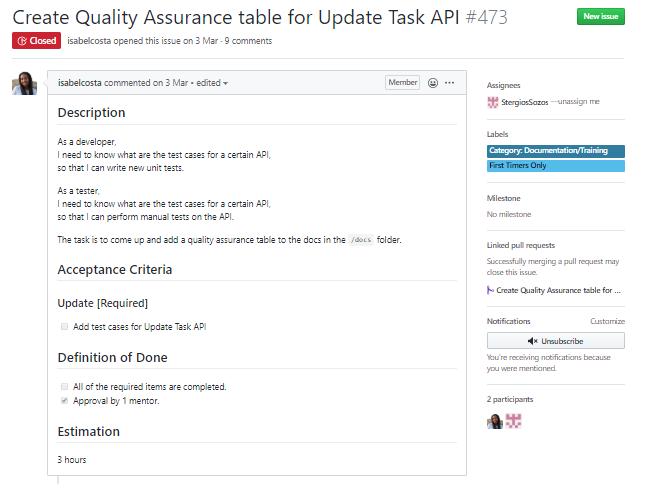
\includegraphics[totalheight=13cm, width=15cm]{issue473.png}}
    \caption{Issue 473}
    \label{fig:verticalcell}
\end{figure}
%-----

\vfill
\clearpage

\subsubsection{Communication with the team}

\hspace{0.5cm}This issue was labeled for first-time contributors so we asked if we could work on this issue to understand the project better. The main maintainer was really helpful and answering out questions soon after we sent them.
Fisrtly, we thought that new unit tests were required, combined with the quallity assurane table, but after our comminucation it was clear to us that only the table had to be completed, as the tests already existed.
While doing this table, by executing some tasks, we found out that there was a possible problem, and an issue had to be raised, as the maintainer agreed.

\subsubsection{Our work}

\hspace{0.5cm}We worked in the default develop branch for this issue. We came to realize that this was a wrong startegy so in all other issues we created a specific branch for them. We tried to write meaningful messages in our commit messages always following the commit style guide suggested by the project. When we thought that the commit message was not understandable enough we wrote a body in our commit messages and documented further our change.

Regarding the way we created the table, firstly we found th file that we had to change, which was easy as the creator of the issue had already mentioned which one is it. Then the difficult part was understanding what exaclty we had to write on the table and how to test it. After going through the test cases to take some ideas on what we could test on the backend server, we tried to create an account on the server. We used temp mail, as it was suggested, and created 4 profiles, so we could test all the possibilities we wanted. For example, we needed a user with a non-verified email, and one with verified. 
Then, we strugled a lot to find out the parameters-arguments that were needed for completing the task we wanted. For example a "token" was required but there was nowhere any explanation about this token. After some searching, we realised that when a user is logging in the server, the success message also provides this token. But even the way that we needed to insert the token was unusual, as we had to write "Bearer <token here>"
Finally, when we had our users ready, and new how to use the backend server, we finallly tested all the scenarios and write them down in the table.

\subsubsection{Testing}
\hspace{0.5cm}Since this change was a change in the UI we did not need to run local testing or write new tests. Instead, our changes were visible in github, as the file was written in markdown language and that's how we verified that our changes were visible and correct. Also, we verified that the continuous integration testing in Travis CI was passing. 
\subsubsection{Code Reviews}
\hspace{0.5cm}Our pull request received immidiate feedback and reviews. our first PR needed some important changes:
1) We were checking multiple failing variables, but only one was required each time. For example we were testing the result of the task with arg1 and arg2 causing the task to fail but arg1 was enough and a separate test for arg2 was required. 
2) We were describing a variable/argument as "wrong" but we did not specify why it was wrong. For example, a user could not exist, or he could have not accepted the terms, or even not verufy his email address. These 3 cases should be separate and specified.
3) We reffered the users with pronouns and we had to make it general ("the user" instead of "he").
4) We had to fix merge conflocts as the PR was approved later.
 Also, other contributors viewed our changes and accepted them. 
\subsubsection{Change}

\subsection{Issue 2 -Fix description messages on Mentorship Relation - \emph{Merged} \#554}
\subsubsection{Issue}
% Image
\begin{figure}[tph!]
\centerline{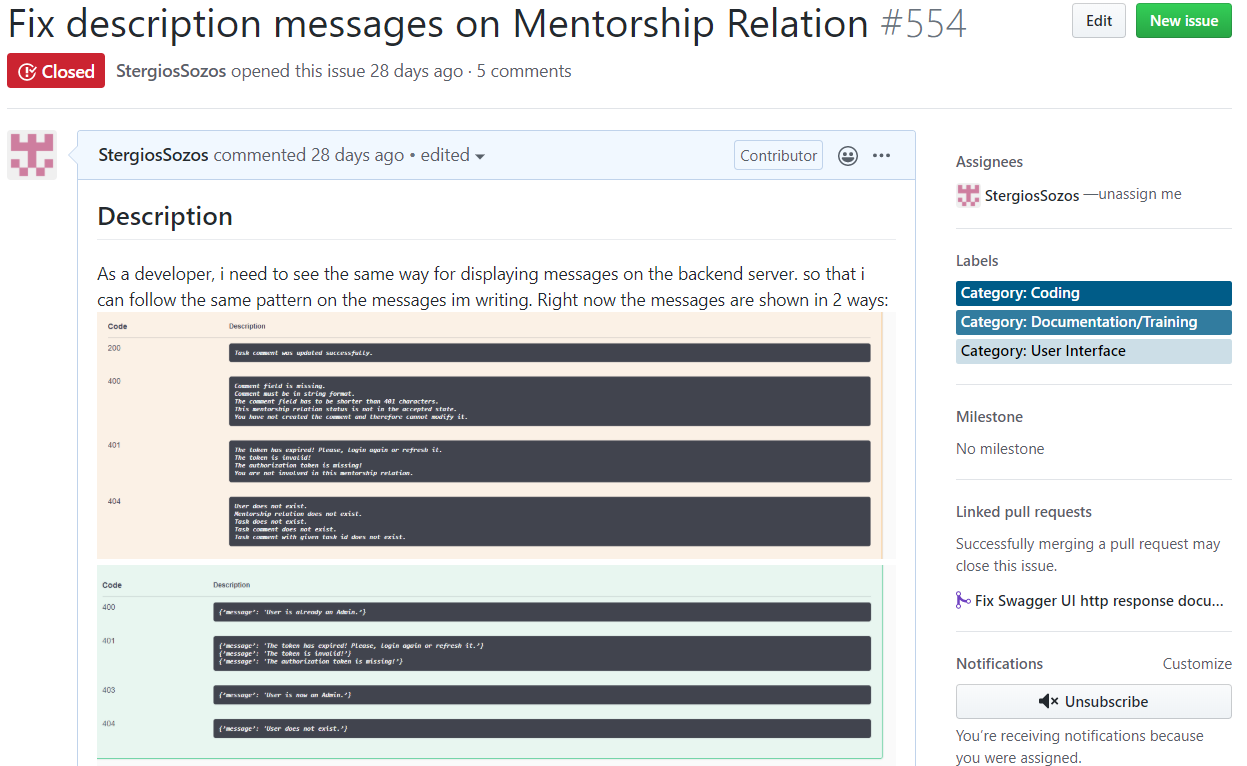
\includegraphics[totalheight=13cm, width=16cm]{issue554part1.png}}
    \caption{Issue 554-1}
    \label{fig:verticalcell}
\end{figure}
%-----

\vfill
\clearpage

\subsubsection{Communication with the team}

\subsubsection{Our work}
\subsubsection{Testing}
\subsubsection{Code Reviews}
\subsubsection{Change}
\subsection{Issue 3 - `Complete task` not including all the necessary information when request id is not in accepted mode - \emph{Accepted} \#537}

\subsubsection{Issue}
% Image
\begin{figure}[tph!]
\centerline{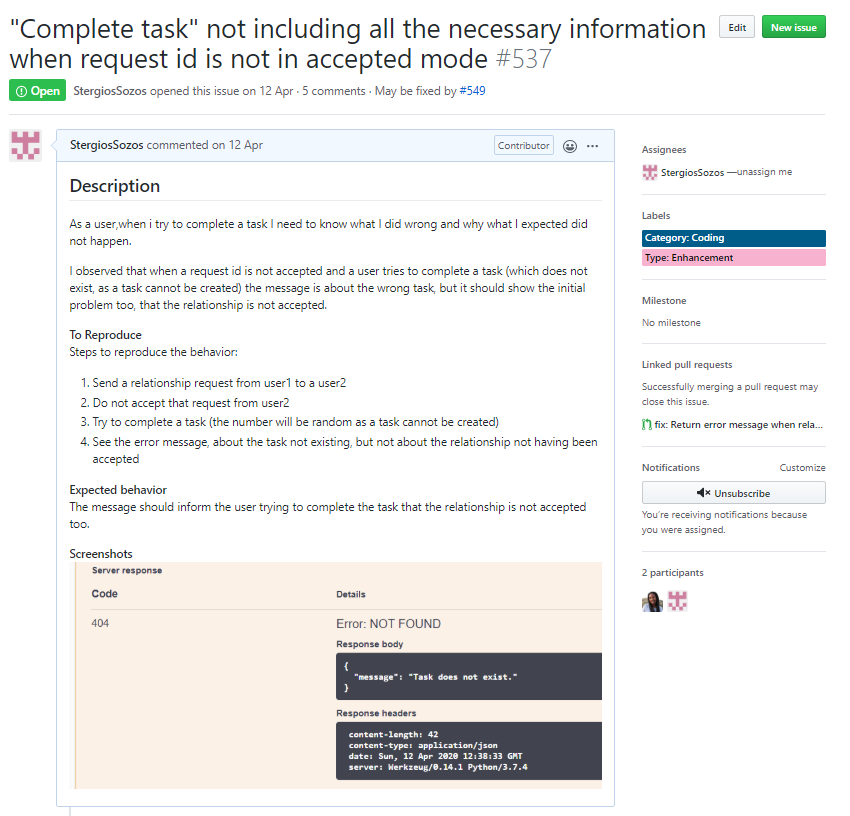
\includegraphics[totalheight=15cm, width=16cm]{issue537.png}}
    \caption{Issue 537}
    \label{fig:verticalcell}
\end{figure}
%-----

\vfill
\clearpage
\subsubsection{Communication with the team}
We had already talked about this issue with the maintainer in a PR, so after the maintainer's approval, we opened a new issue, and got assigned to it. We also clarified, that the solution suggested on this issue, is giving higher priority to a specific argument, whih was the state of the relationship status, instead of the one that was then highest, which was the existence of the task.

\subsubsection{Our work}

We added an if statement before the existings one, so that it will be prioratized, and included the new possible responses on the responses board on the backend server. After that we changed the hardcoded status (i.e. 400,401 etc) to http status. Then, we changed the way messages were printed into f strings and added some blank spaces that were needed. Finally, we wrote a unit test for the added if statement.

After the original 
\subsubsection{Testing}
Initially, we didn't have any unit testing for the speific change, and we tested it only on the backend server, and we also confirmed that the continuous integration testing in Travis CI was passing. 
After our PR was reviewed and after all the changes requested had been done, an additional test was asked, a unit test. To create this, we needed to also add a user to the database and create a new relation of this user with another user.

\subsubsection{Code Reviews}
The main part of the PR was approved, and only some minor changes were asked, regarding new standards(http status instead of harcoded numbers, f strings for printing messages) and a blank line to separate visually validation sections. After these minor changes, a unit test was asked.
\subsubsection{Change}

\subsection{Issue 4 - Title of issue to be added}
Pull Request - Efi


\subsubsection{Issue}
A section

\subsubsection{Communication with the team}
A section

\subsubsection{More subsections}
A section

\subsection{Issue 5 - Title of issue to be added}
Pull Request - Efi

\subsubsection{Issue}
A section

\subsubsection{Communication with the team}
A section

\subsubsection{More subsections}
A section

\subsection{Issue 6 - Title of issue to be added}
Pull Request - Efi

\subsubsection{Issue}
A section

\subsubsection{Communication with the team}
A section

\subsubsection{More subsections}
A section
\subsection{Issue 7 - Title of issue to be added}
Pull Request - Efi

\subsubsection{Issue}
A section

\subsubsection{Communication with the team}
A section

\subsubsection{More subsections}
A section

\section{Conclusion}
Contributing to an open-source project
 enriched our understanding  of program 
development and urged us to try to establish 
possible improvements. We were able to express
 our opinion with facts and use the terminology we
 learned during the course. We researched a lot with
 or without the guidance of the open-source community
 and offered feasible solutions. In the future, we want
 to continue contributing to other open-source projects.
\section*{References}
[1] https://github.com/anitab-org
\newline
[2] https://github.com/anitab-org/mentorship-android
\newline
[3] https://github.com/anitab-org/mentorship-backend
\end{document}